% Standalone TikZ skeleton for Figure 1 (UMA-Inverse architecture).
%
% Compile with: pdflatex fig1_architecture.tex
% (no bibliography, no class dependencies)
%
% Three panels:
%   (a) PairMixer encoder block + decoding head
%   (b) Pair-tensor block decomposition: [L,L] / [L,M] / [M,M]
%   (c) v1 -> v2 featurizer changes
%
% Sizing tuned for a single-column bioRxiv figure (~7 cm wide per panel).
% Tweak coordinates / colors freely; this is a starting point, not a final.

\documentclass[tikz,border=4pt]{standalone}
\usepackage{amsmath}
\usepackage{amssymb}
\usepackage{tikz}
\usetikzlibrary{positioning,arrows.meta,shapes.geometric,fit,backgrounds,calc}

% --- shared style -----------------------------------------------------------
\tikzset{
  node distance=4mm and 6mm,
  every node/.style={font=\footnotesize, align=center},
  block/.style={
    draw, rounded corners=2pt, thick,
    minimum height=8mm, minimum width=22mm,
    fill=blue!6
  },
  feat/.style={
    draw, rounded corners=2pt,
    minimum height=6mm, minimum width=14mm,
    fill=gray!10, font=\scriptsize
  },
  pairblock/.style={
    draw, thick,
    minimum height=18mm, minimum width=18mm
  },
  arrow/.style={-{Latex[length=2mm]}, thick},
  panellabel/.style={font=\bfseries, anchor=north west}
}

\begin{document}
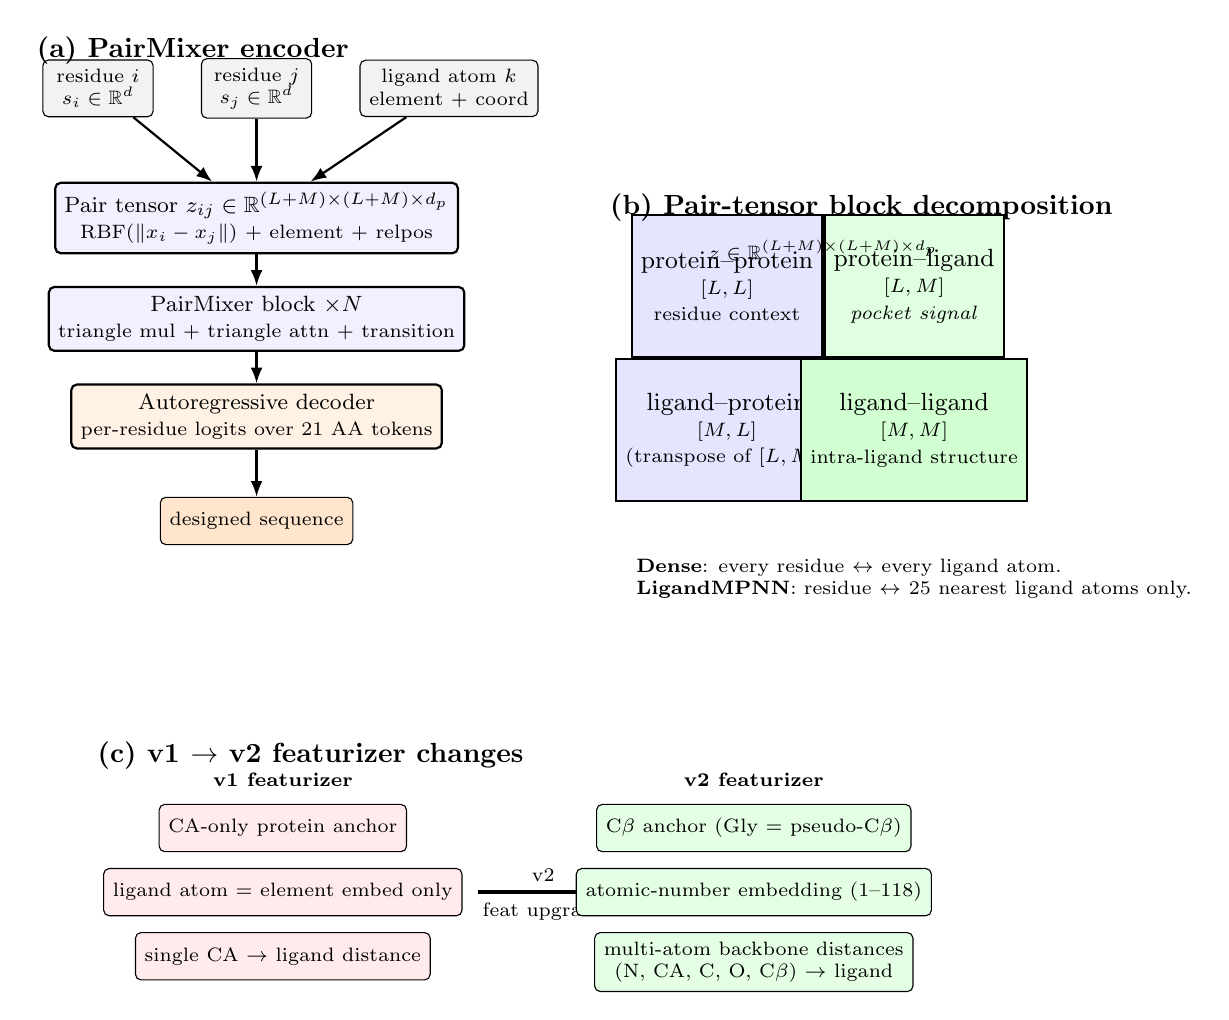
\begin{tikzpicture}

%% ===========================================================================
%% Panel (a): PairMixer encoder block
%% ===========================================================================
\begin{scope}[local bounding box=panelA]

  % inputs
  \node[feat]                      (resi)  {residue $i$\\\scriptsize $s_i \in \mathbb{R}^{d}$};
  \node[feat, right=of resi]       (resj)  {residue $j$\\\scriptsize $s_j \in \mathbb{R}^{d}$};
  \node[feat, right=of resj]       (atomk) {ligand atom $k$\\\scriptsize element + coord};

  % pair-tensor formation
  \node[block, below=8mm of resj]  (pair)  {Pair tensor $z_{ij} \in \mathbb{R}^{(L+M) \times (L+M) \times d_p}$\\\scriptsize RBF($\|x_i - x_j\|$) + element + relpos};

  \draw[arrow] (resi)  -- (pair);
  \draw[arrow] (resj)  -- (pair);
  \draw[arrow] (atomk) -- (pair);

  % stack of N PairMixer blocks
  \node[block, below=of pair]      (pm1)   {PairMixer block $\times N$\\\scriptsize triangle mul + triangle attn + transition};
  \draw[arrow] (pair) -- (pm1);

  % decoding head
  \node[block, below=of pm1, fill=orange!10] (head) {Autoregressive decoder\\\scriptsize per-residue logits over 21 AA tokens};
  \draw[arrow] (pm1) -- (head);

  % output
  \node[feat, below=6mm of head, fill=orange!20] (seq) {designed sequence};
  \draw[arrow] (head) -- (seq);

  % panel label
  \node[panellabel] at ($(panelA.north west) + (-2mm, 4mm)$) {(a) PairMixer encoder};

\end{scope}

%% ===========================================================================
%% Panel (b): Pair-tensor block decomposition
%% ===========================================================================
\begin{scope}[shift={($(panelA.east) + (24mm, 0)$)}, local bounding box=panelB]

  % the [L+M, L+M] tensor as a 2x2 block matrix
  \node[pairblock, fill=blue!10] (LL) at (0, 0)     {{\small protein--protein}\\\scriptsize $[L, L]$\\\scriptsize residue context};
  \node[pairblock, fill=green!12, right=0mm of LL] (LM) {{\small protein--ligand}\\\scriptsize $[L, M]$\\\scriptsize \emph{pocket signal}};
  \node[pairblock, fill=blue!10, below=0mm of LL] (ML) {{\small ligand--protein}\\\scriptsize $[M, L]$\\\scriptsize (transpose of $[L,M]$)};
  \node[pairblock, fill=green!18, below=0mm of LM] (MM) {{\small ligand--ligand}\\\scriptsize $[M, M]$\\\scriptsize intra-ligand structure};

  % outer label
  \node[above=2mm of $(LL.east)!0.5!(LM.west)$, font=\scriptsize] {$z \in \mathbb{R}^{(L+M)\times(L+M)\times d_p}$};

  % key contrast vs LigandMPNN
  \node[below=6mm of MM, font=\scriptsize, align=left, anchor=north]
    {\textbf{Dense}: every residue $\leftrightarrow$ every ligand atom.\\
     \textbf{LigandMPNN}: residue $\leftrightarrow$ 25 nearest ligand atoms only.};

  \node[panellabel] at ($(panelB.north west) + (-2mm, 4mm)$) {(b) Pair-tensor block decomposition};

\end{scope}

%% ===========================================================================
%% Panel (c): v1 -> v2 featurizer changes
%% ===========================================================================
\begin{scope}[shift={($(panelA.south) + (0, -36mm)$)}, local bounding box=panelC]

  % v1 column
  \node[feat, fill=red!8]                             (v1a) {CA-only protein anchor};
  \node[feat, fill=red!8, below=2mm of v1a]            (v1b) {ligand atom = element embed only};
  \node[feat, fill=red!8, below=2mm of v1b]            (v1c) {single CA $\rightarrow$ ligand distance};

  \node[above=1mm of v1a, font=\scriptsize\bfseries] {v1 featurizer};

  % arrow
  \node[right=14mm of v1b] (arrowmid) {};
  \draw[arrow, very thick] ($(v1b.east) + (2mm, 0)$) -- ($(arrowmid.east) + (2mm, 0)$)
    node[midway, above, font=\scriptsize] {v2}
    node[midway, below, font=\scriptsize] {feat upgrade};

  % v2 column
  \node[feat, fill=green!10, right=24mm of v1a]        (v2a) {C$\beta$ anchor (Gly = pseudo-C$\beta$)};
  \node[feat, fill=green!10, below=2mm of v2a]         (v2b) {atomic-number embedding (1--118)};
  \node[feat, fill=green!10, below=2mm of v2b]         (v2c) {multi-atom backbone distances\\\scriptsize (N, CA, C, O, C$\beta$) $\rightarrow$ ligand};

  \node[above=1mm of v2a, font=\scriptsize\bfseries] {v2 featurizer};

  \node[panellabel] at ($(panelC.north west) + (-2mm, 4mm)$) {(c) v1 $\rightarrow$ v2 featurizer changes};

\end{scope}

\end{tikzpicture}
\end{document}
